\chapter{EMPATÍA}
El presente capítulo desarrolla la primera etapa del Design Thinking aplicada al presente proyecto: Empatizar. Esta fase tiene como propósito comprender en profundidad las necesidades, motivaciones y frustraciones de los jóvenes respecto a su experiencia con las redes sociales y la conexión emocional digital, complementando la evidencia documental presentada en el Capítulo 3 con evidencia primaria recolectada directamente del grupo objetivo. Para ello se aplicaron tres técnicas: una guía de entrevista cualitativa semiestructurada, la aplicación de dicha entrevista a seis participantes, y la Técnica de los 5 ¿Por qué? para profundizar en las causas raíz de los problemas identificados.

\section{GUÍA DE LA ENTREVISTA CUALITATIVA}
Con el objetivo de establecer una guía de apoyo para el desarrollo de las entrevistas, se elaboró un guion estructurado en tres momentos: introducción, preguntas personales, y dos bloques temáticos centrales (redes sociales y bienestar emocional), cerrando con una conclusión. El diseño de este instrumento se fundamentó en los factores de desconexión emocional identificados en el Capítulo 3, particularmente aquellos vinculados al tipo de interacción digital (Godard \& Holtzman, 2024; Liu et al., 2026) y a la discrepancia entre conexión cuantitativa y vínculo significativo (Smith et al., 2021).

\subsection{Introducción}
Al inicio de cada entrevista se explicó el propósito del estudio, se solicitó el consentimiento para la grabación de la sesión y se enfatizó la confidencialidad de la información compartida por los participantes.

\subsection{Preguntas personales}
\begin{itemize}
    \item ¿Cuál es tu nombre y edad?
    \item ¿A qué te dedicas actualmente (estudias, trabajas, ambas)?
    \item ¿Cuáles son las redes sociales o apps de mensajería que más usas en tu día a día?
    \item ¿Aproximadamente cuántas horas al día pasas en redes sociales?
\end{itemize}

\subsection{Redes sociales}
\begin{itemize}
    \item ¿Sientes que la mayoría del tiempo estás interactuando con otras personas o más bien viendo contenido sin interactuar?
    \item ¿Puedes contarme sobre alguna vez que una interacción en redes sociales te haya hecho sentir realmente bien o conectado con alguien?
    \item ¿Y alguna vez que te haya hecho sentir mal, comparado(a), o más solo(a) de lo que ya estabas?
    \item ¿Qué opinas sobre los likes, seguidores o vistas? ¿Sientes que te generan algún tipo de presión o comparación?
    \item De tus contactos digitales, ¿cuántos dirías que son vínculos realmente significativos para ti?
    \item Si pudieras cambiar algo de cómo funcionan las redes sociales actuales, ¿qué cambiarías?
    \item Si tuvieras que enviar solo unos pocos mensajes breves al día a alguien nuevo, ¿sentirías que es más fácil o significativo si esa persona comparte algún interés contigo, o preferirías que sea totalmente al azar? ¿Por qué?
    \item Si tuvieras que personalizar cómo te representas en una app, por ejemplo con un avatar en vez de una foto real, ¿qué tan importante sería eso para ti?
    \item ¿Qué tan cómodo(a) te sentirías conversando con una persona que no conoces, aunque sea de forma anónima o con avatar? ¿Qué te generaría más confianza?
\end{itemize}

\subsection{Bienestar emocional}
\begin{itemize}
    \item ¿Sientes que tienes suficientes personas con quienes hablar cuando necesitas apoyo?
    \item ¿Alguna vez has sentido que, a pesar de tener muchos contactos digitales, te sientes solo(a)?
    \item ¿Qué tipo de mensajes o gestos de otras personas te hacen sentir realmente acompañado(a) o valorado(a)?
    \item ¿Prefieres conversaciones largas y poco frecuentes, o mensajes breves pero más constantes? ¿Por qué?
    \item Cuando algo bueno te pasa en el día, ¿sueles compartirlo con alguien? ¿Con quién y por qué medio?
    \item Si existiera una app pensada exclusivamente para enviar y recibir mensajes breves y positivos entre personas, sin likes ni seguidores públicos, ¿qué esperarías de ella? ¿La usarías?
    \item ¿Hay algún tipo de mensaje o palabra que te gustaría recibir más seguido, pero que sientes que casi nunca recibes?
    \item Si usaras esta app, ¿cuántos mensajes o interacciones esperarías tener al día?
\end{itemize}

\subsection{Conclusión}
Se agradeció la participación y disposición de cada entrevistado, dando espacio a comentarios adicionales antes de finalizar la sesión.

\section{APLICACIÓN DE LAS ENTREVISTAS}
La guía descrita fue aplicada a seis jóvenes de entre 16 y 28 años (Usuario 1: Rolando Mercado Rojas, Usuario 2: Rubén Hernández Torrez, Usuario 3: Fernando José Pérez Armando, Usuario 4: Antonia Tapia, Usuario 5: Alejandra Pérez Ramal, Usuario 6: Renata Martínez Mitte), residentes en Cochabamba, Bolivia, reclutados a través de grupos digitales de contacto directo con el grupo objetivo. El criterio de selección priorizó la diversidad de perfiles (género, nivel de sociabilidad autopercibido) con el fin de enriquecer los hallazgos cualitativos, en línea con la recomendación de incorporar diversidad de perspectivas al construir mapas de empatía (Vargas Márquez et al., 2021). Las entrevistas tuvieron una duración aproximada de 20 a 30 minutos cada una, y sus resultados fueron sistematizados utilizando la técnica de Entrevistas Cualitativas de Design Thinking, organizada en cuatro categorías: necesidades, problemas, deseos y observaciones.

A continuación, se presentan de forma detallada los resultados de los Usuarios 1 y 4, seleccionados por representar perfiles contrastantes dentro de la muestra (un perfil introvertido con dificultad de vinculación frente a uno sociable con red de apoyo consolidada), lo cual permite ilustrar la amplitud de experiencias recogidas.

\subsection{Usuario 1: Rolando Mercado Rojas}
Rolando, de 25 años, estudiante universitario, presenta un uso moderado de redes sociales (1 a 2 horas diarias). Se define a sí mismo como una persona reservada e introspectiva, con dificultad para iniciar y mantener conversaciones tanto digitales como presenciales.

\begin{figure}[htbp]
  \centering
  \caption{Entrevista cualitativa - Usuario 1 (Rolando Mercado Rojas)}
  \label{fig:entrevista_usuario1}
  \vspace{4pt}
  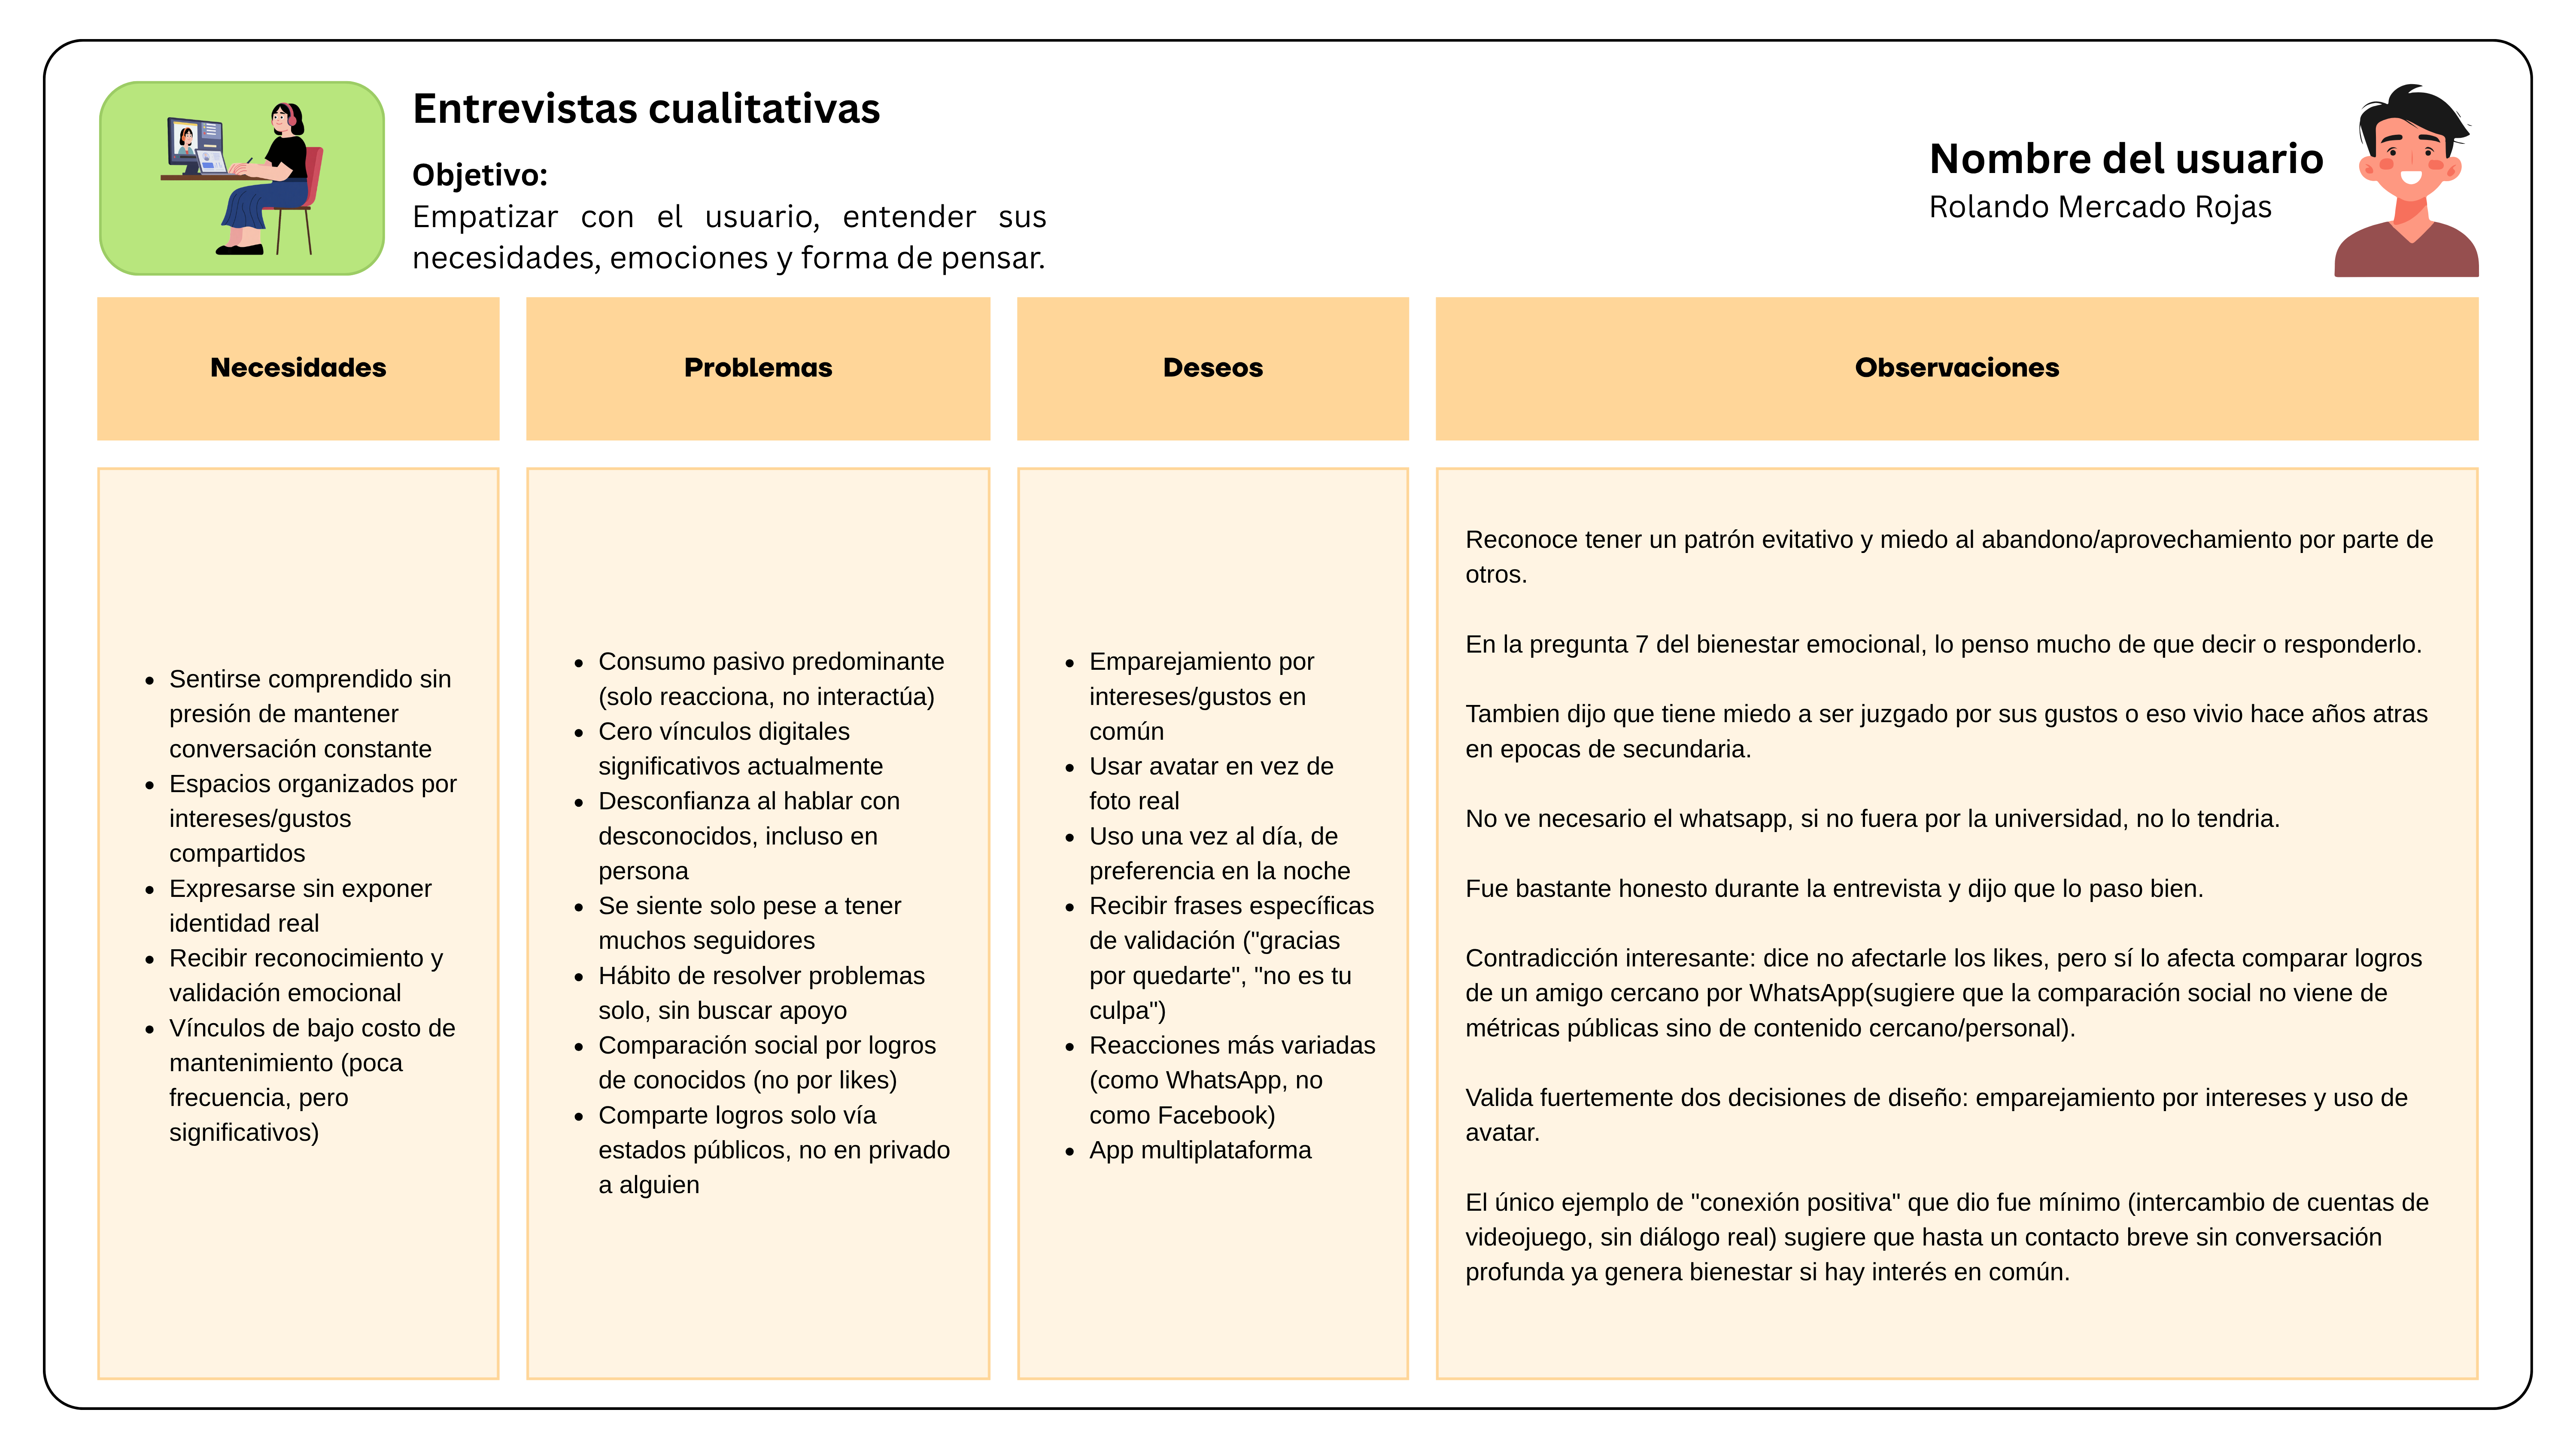
\includegraphics[width=0.9\textwidth]{Images/methodology/empathy/usuario1EC.png}
  \vspace{4pt}
\end{figure}

Entre los hallazgos más relevantes de esta entrevista destaca que Rolando no identifica ningún vínculo digital que considere significativo, pese a contar con un número considerable de seguidores en redes sociales, lo que evidencia la discrepancia entre conexión cuantitativa y vínculo cualitativo señalada por Smith et al. (2021) y por el modelo de vinculación social ligera y elaborada propuesto por Takano (2018). Asimismo, valida fuertemente dos decisiones de diseño relevantes para el presente proyecto: la preferencia por el emparejamiento basado en intereses compartidos, consistente con los hallazgos de Liu et al. (2026) sobre el rol del canal y contenido de la comunicación en la asociación entre redes sociales y aislamiento social, y el uso de un avatar en lugar de una fotografía real como medio de expresión.

\subsection{Usuario 4: Antonia Tapia}
Antonia, de 20 años, estudiante, presenta un uso considerable de redes sociales (3 horas diarias). A diferencia de Rolando, cuenta con una red de apoyo sólida y vínculos significativos ya establecidos, mostrando un perfil más sociable, aunque igualmente crítico frente a las dinámicas actuales de las redes sociales.

\begin{figure}[htbp]
  \centering
  \caption{Entrevista cualitativa - Usuario 4 (Antonia Tapia)}
  \label{fig:entrevista_usuario4}
  \vspace{4pt}
  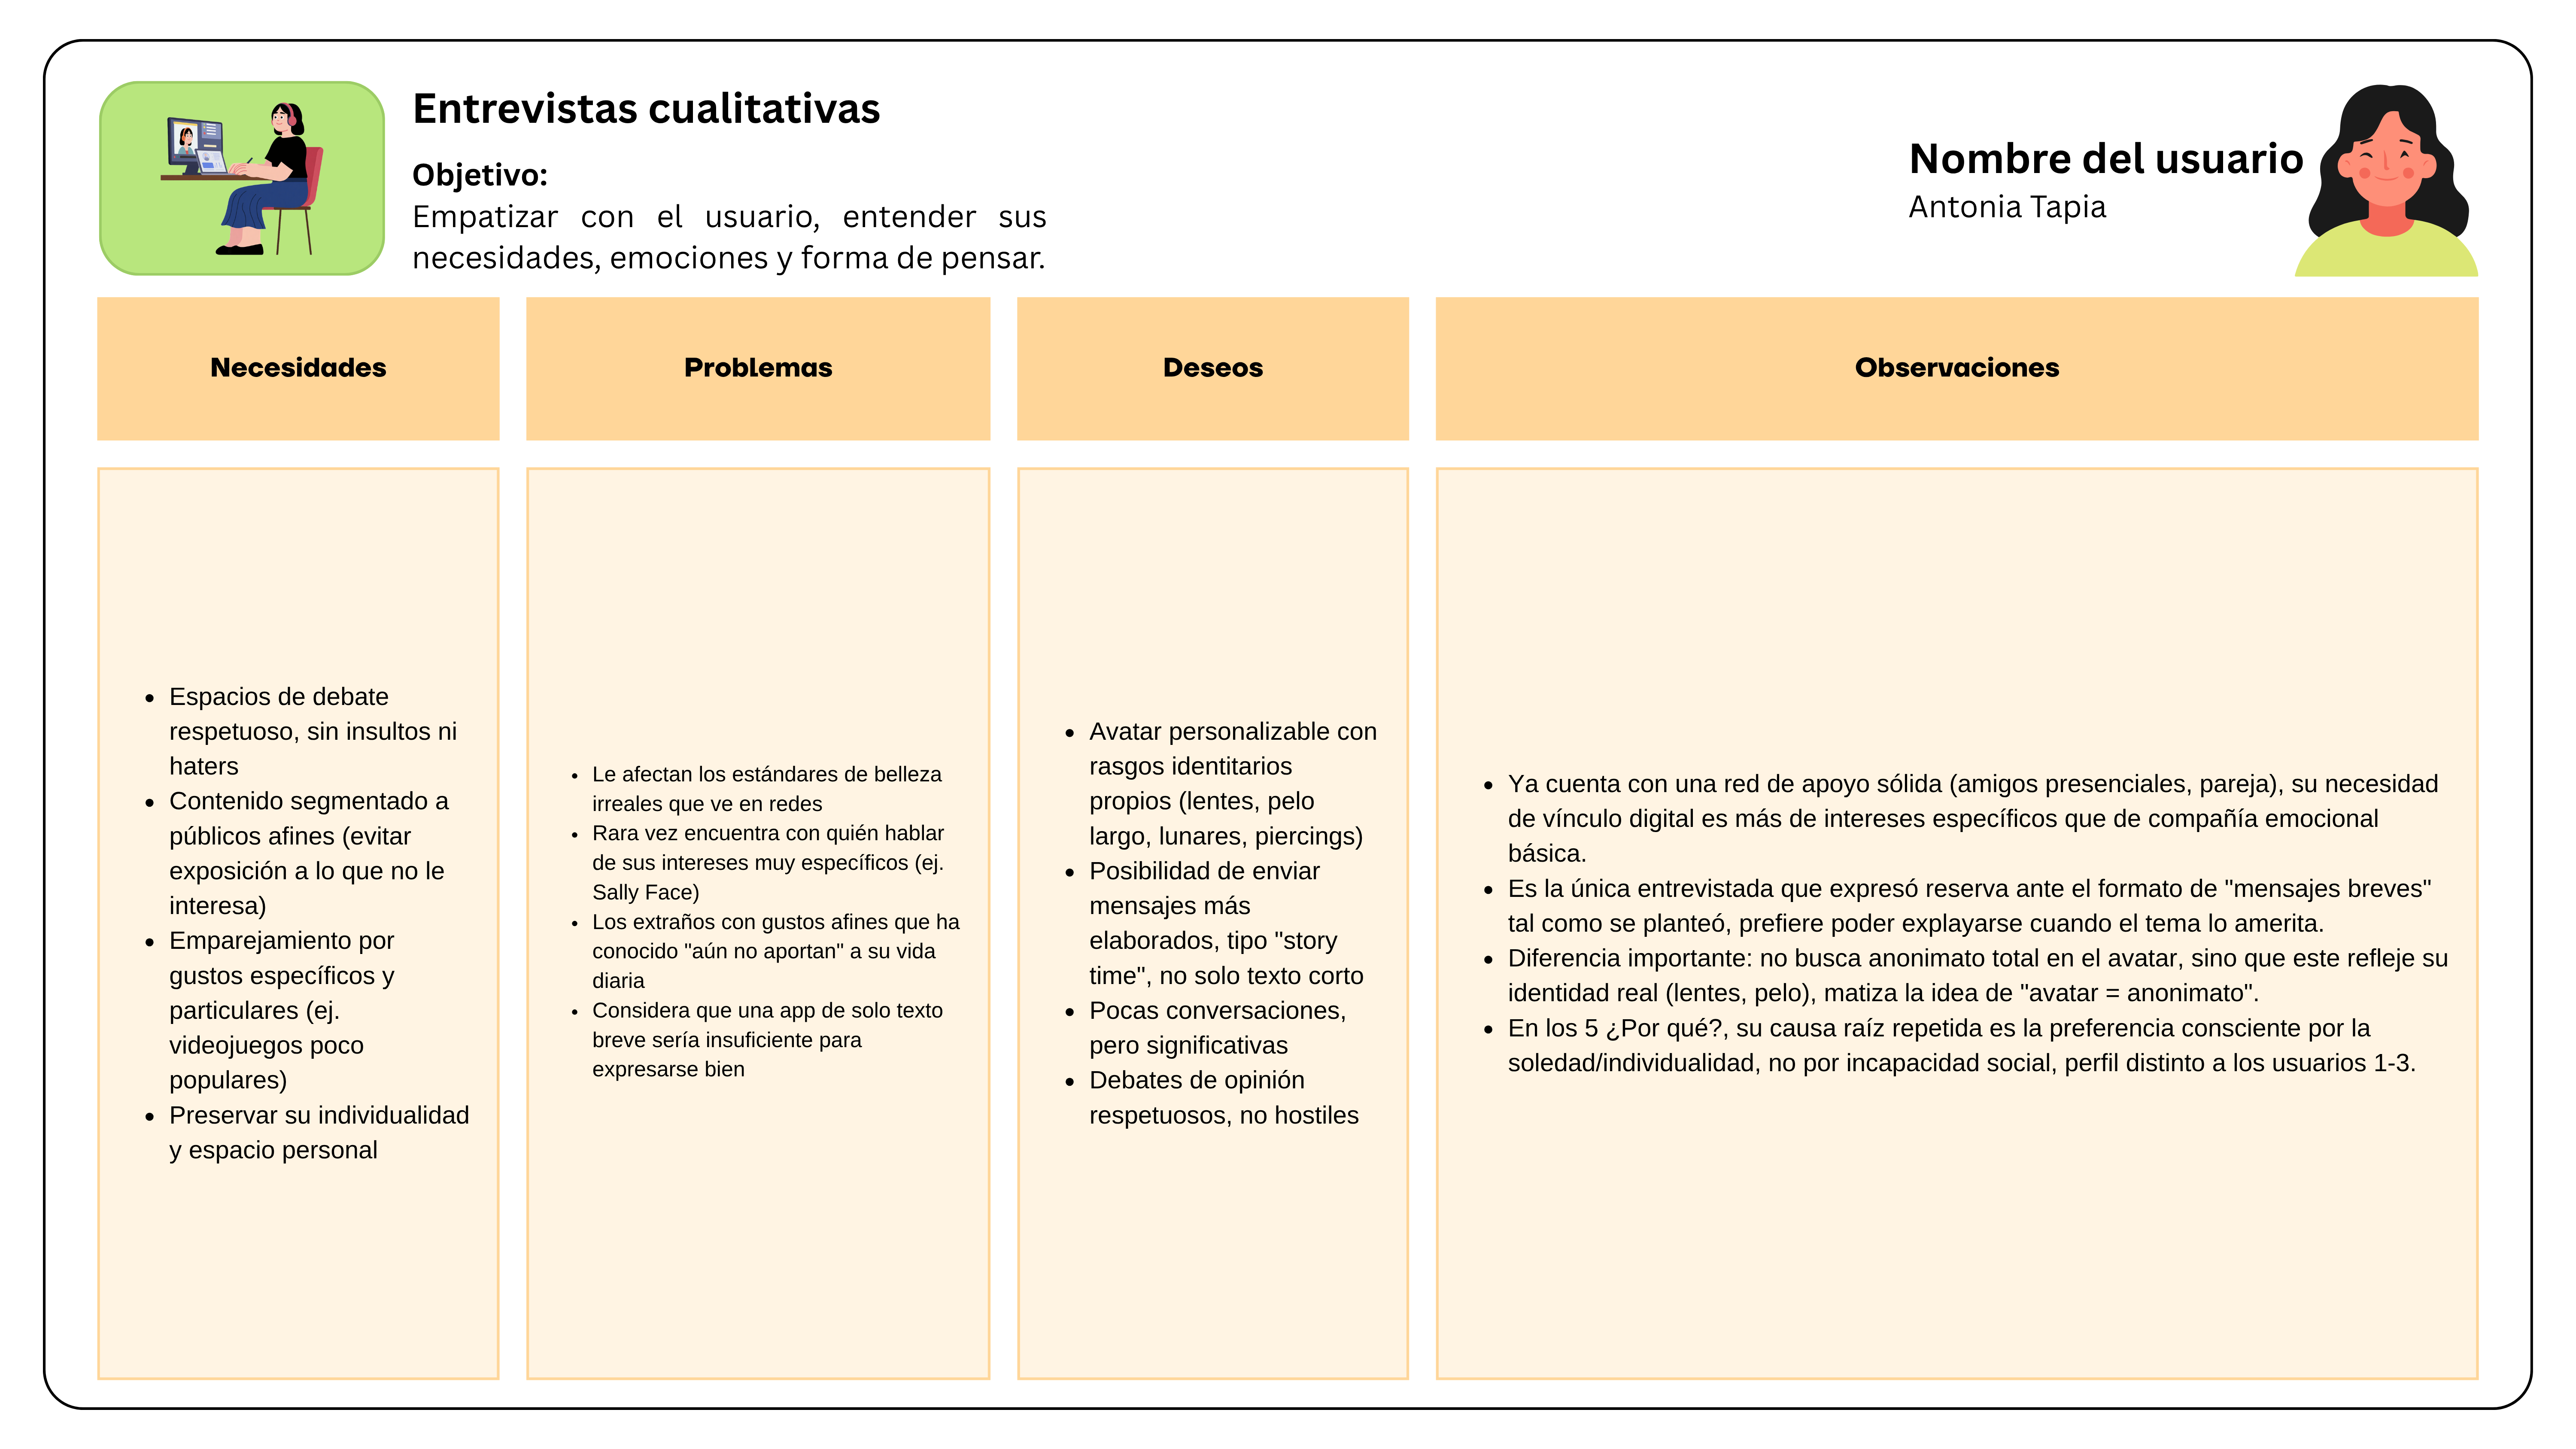
\includegraphics[width=0.9\textwidth]{Images/methodology/empathy/usuario4EC.png}
  \vspace{4pt}
\end{figure}

Antonia expresó reservas respecto al formato de mensajes exclusivamente breves, señalando que en ocasiones necesita mayor espacio para expresarse. Este hallazgo resulta relevante frente al concepto de micro interacciones sociales positivas de Saffer (2013), pues sugiere que la brevedad, si bien valiosa como principio general, no debe aplicarse de forma rígida para todos los perfiles de usuario. Asimismo, destacó la importancia de que el avatar refleje rasgos identitarios reales, matizando la idea inicial de que el avatar debía funcionar como anonimato total.

\subsection{Usuarios 2, 3, 5 y 6}
De manera complementaria, el mismo instrumento fue aplicado a los Usuarios 2 (Rubén Hernández Torrez), 3 (Fernando José Pérez Armando), 5 (Alejandra Pérez Ramal) y 6 (Renata Martínez Mitte). De forma consistente con los Usuarios 1 y 4, estos cuatro participantes reportaron dificultades para sostener vínculos digitales significativos —coincidiendo con el patrón de soledad juvenil creciente documentado por Twenge et al. (2021) y por el meta-análisis de Feng et al. (2026), según el cual la asociación entre redes sociales y soledad depende más del tipo de uso que del tiempo de exposición—, así como preocupación por la hostilidad o desconfianza hacia desconocidos en línea, y una valoración positiva hacia el emparejamiento por intereses compartidos y el uso de avatares como medio de expresión.

\section{TÉCNICA DE LOS 5 ¿POR QUÉ?}
Con el objetivo de profundizar en las causas raíz de los problemas identificados durante las entrevistas, se aplicó la Técnica de los 5 ¿Por qué? a cuatro problemas recurrentes: la soledad pese a tener múltiples contactos digitales, el predominio del consumo pasivo sobre la interacción activa, la comparación social generada por likes y seguidores, y la dificultad para generar conversaciones significativas con desconocidos. Esta técnica permitió superar la descripción superficial de los síntomas para llegar a explicaciones más profundas, en coherencia con el enfoque de inmersión propuesto por Vargas Márquez et al. (2021) para la etapa de empatizar.

A continuación, se presentan los resultados detallados de los Usuarios 1 y 5, seleccionados por ilustrar dos causas raíz distintas y complementarias entre sí.

\subsection{Usuario 1: Rolando Mercado Rojas}
\begin{figure}[htbp]
  \centering
  \caption{Técnica de los 5 ¿Por qué? - Usuario 1 (Rolando Mercado Rojas)}
  \label{fig:5porque_usuario1}
  \vspace{4pt}
  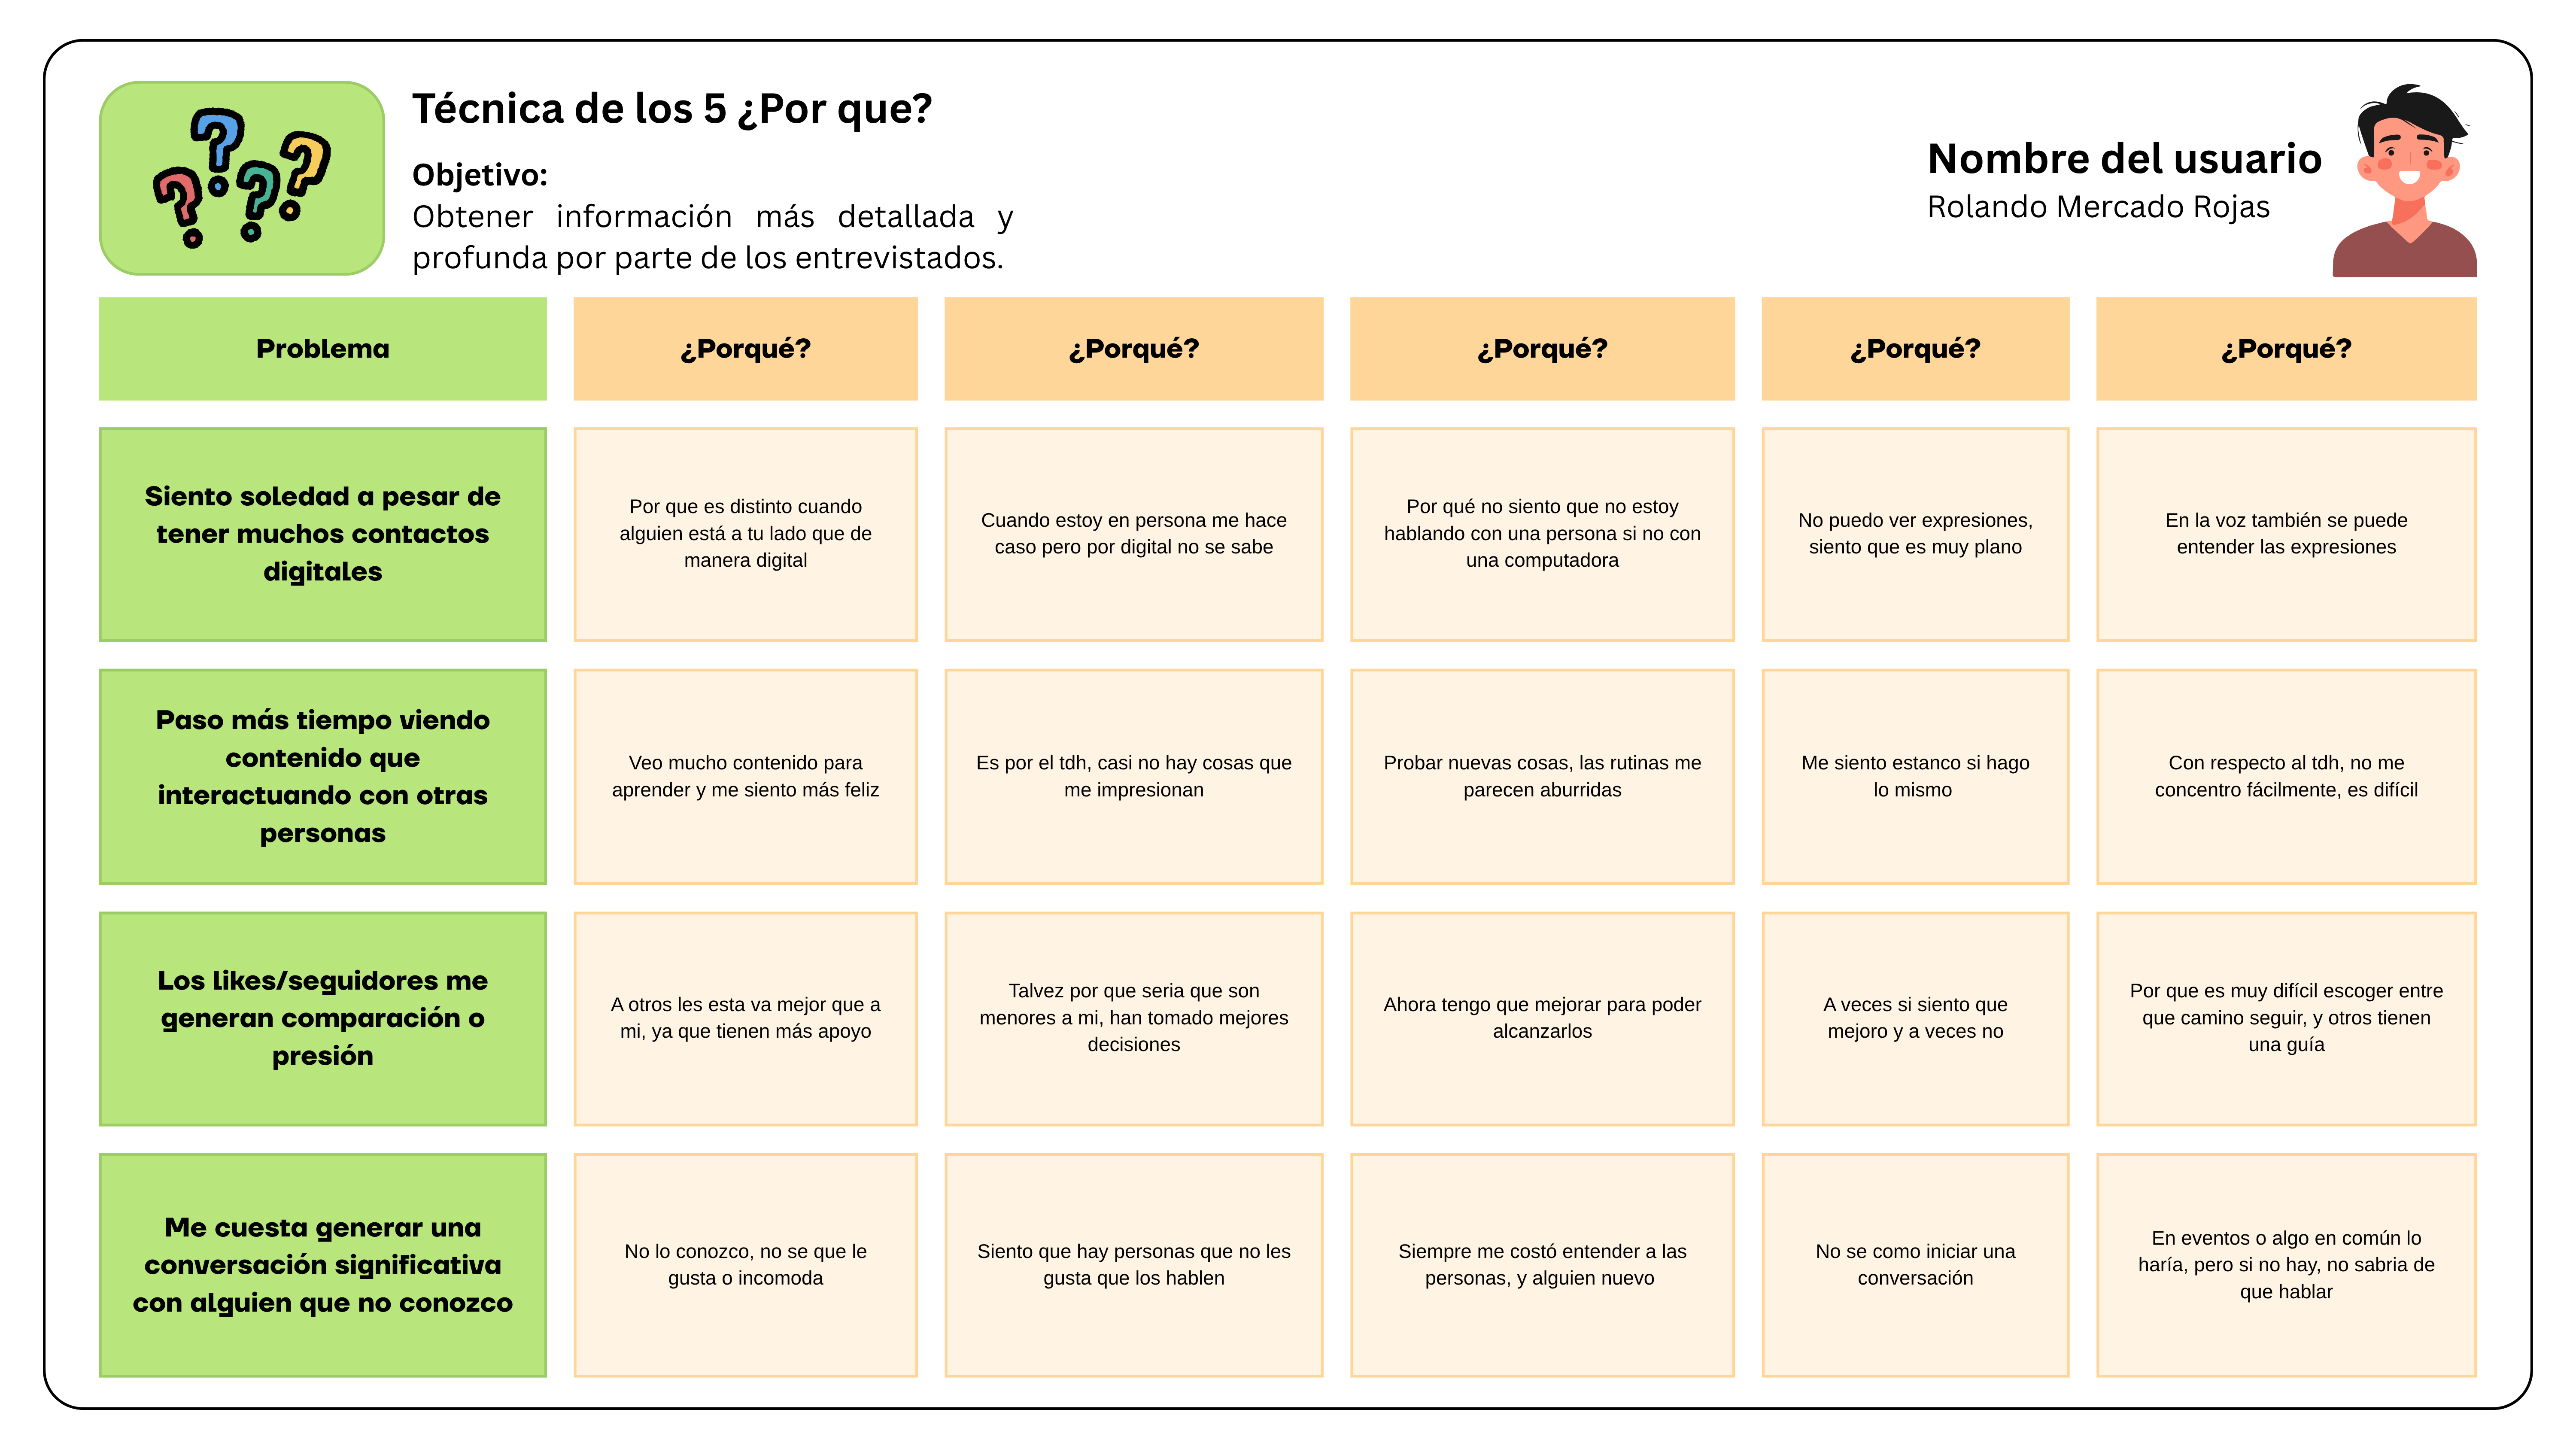
\includegraphics[width=0.9\textwidth]{Images/methodology/empathy/usuario1-5P.png}
  \vspace{4pt}
\end{figure}

El análisis reveló que, para Rolando, la causa raíz de la desconexión digital radica en la ausencia de señales no verbales en la comunicación en línea, lo que hace que la interacción se perciba como poco genuina en comparación con el contacto presencial. Este hallazgo confirma empíricamente la advertencia de Picard (1997) respecto al empobrecimiento del canal emocional en la comunicación mediada por texto.

\subsection{Usuario 5: Alejandra Pérez Ramal}
\begin{figure}[htbp]
  \centering
  \caption{Técnica de los 5 ¿Por qué? - Usuario 5 (Alejandra Pérez Ramal)}
  \label{fig:5porque_usuario5}
  \vspace{4pt}
  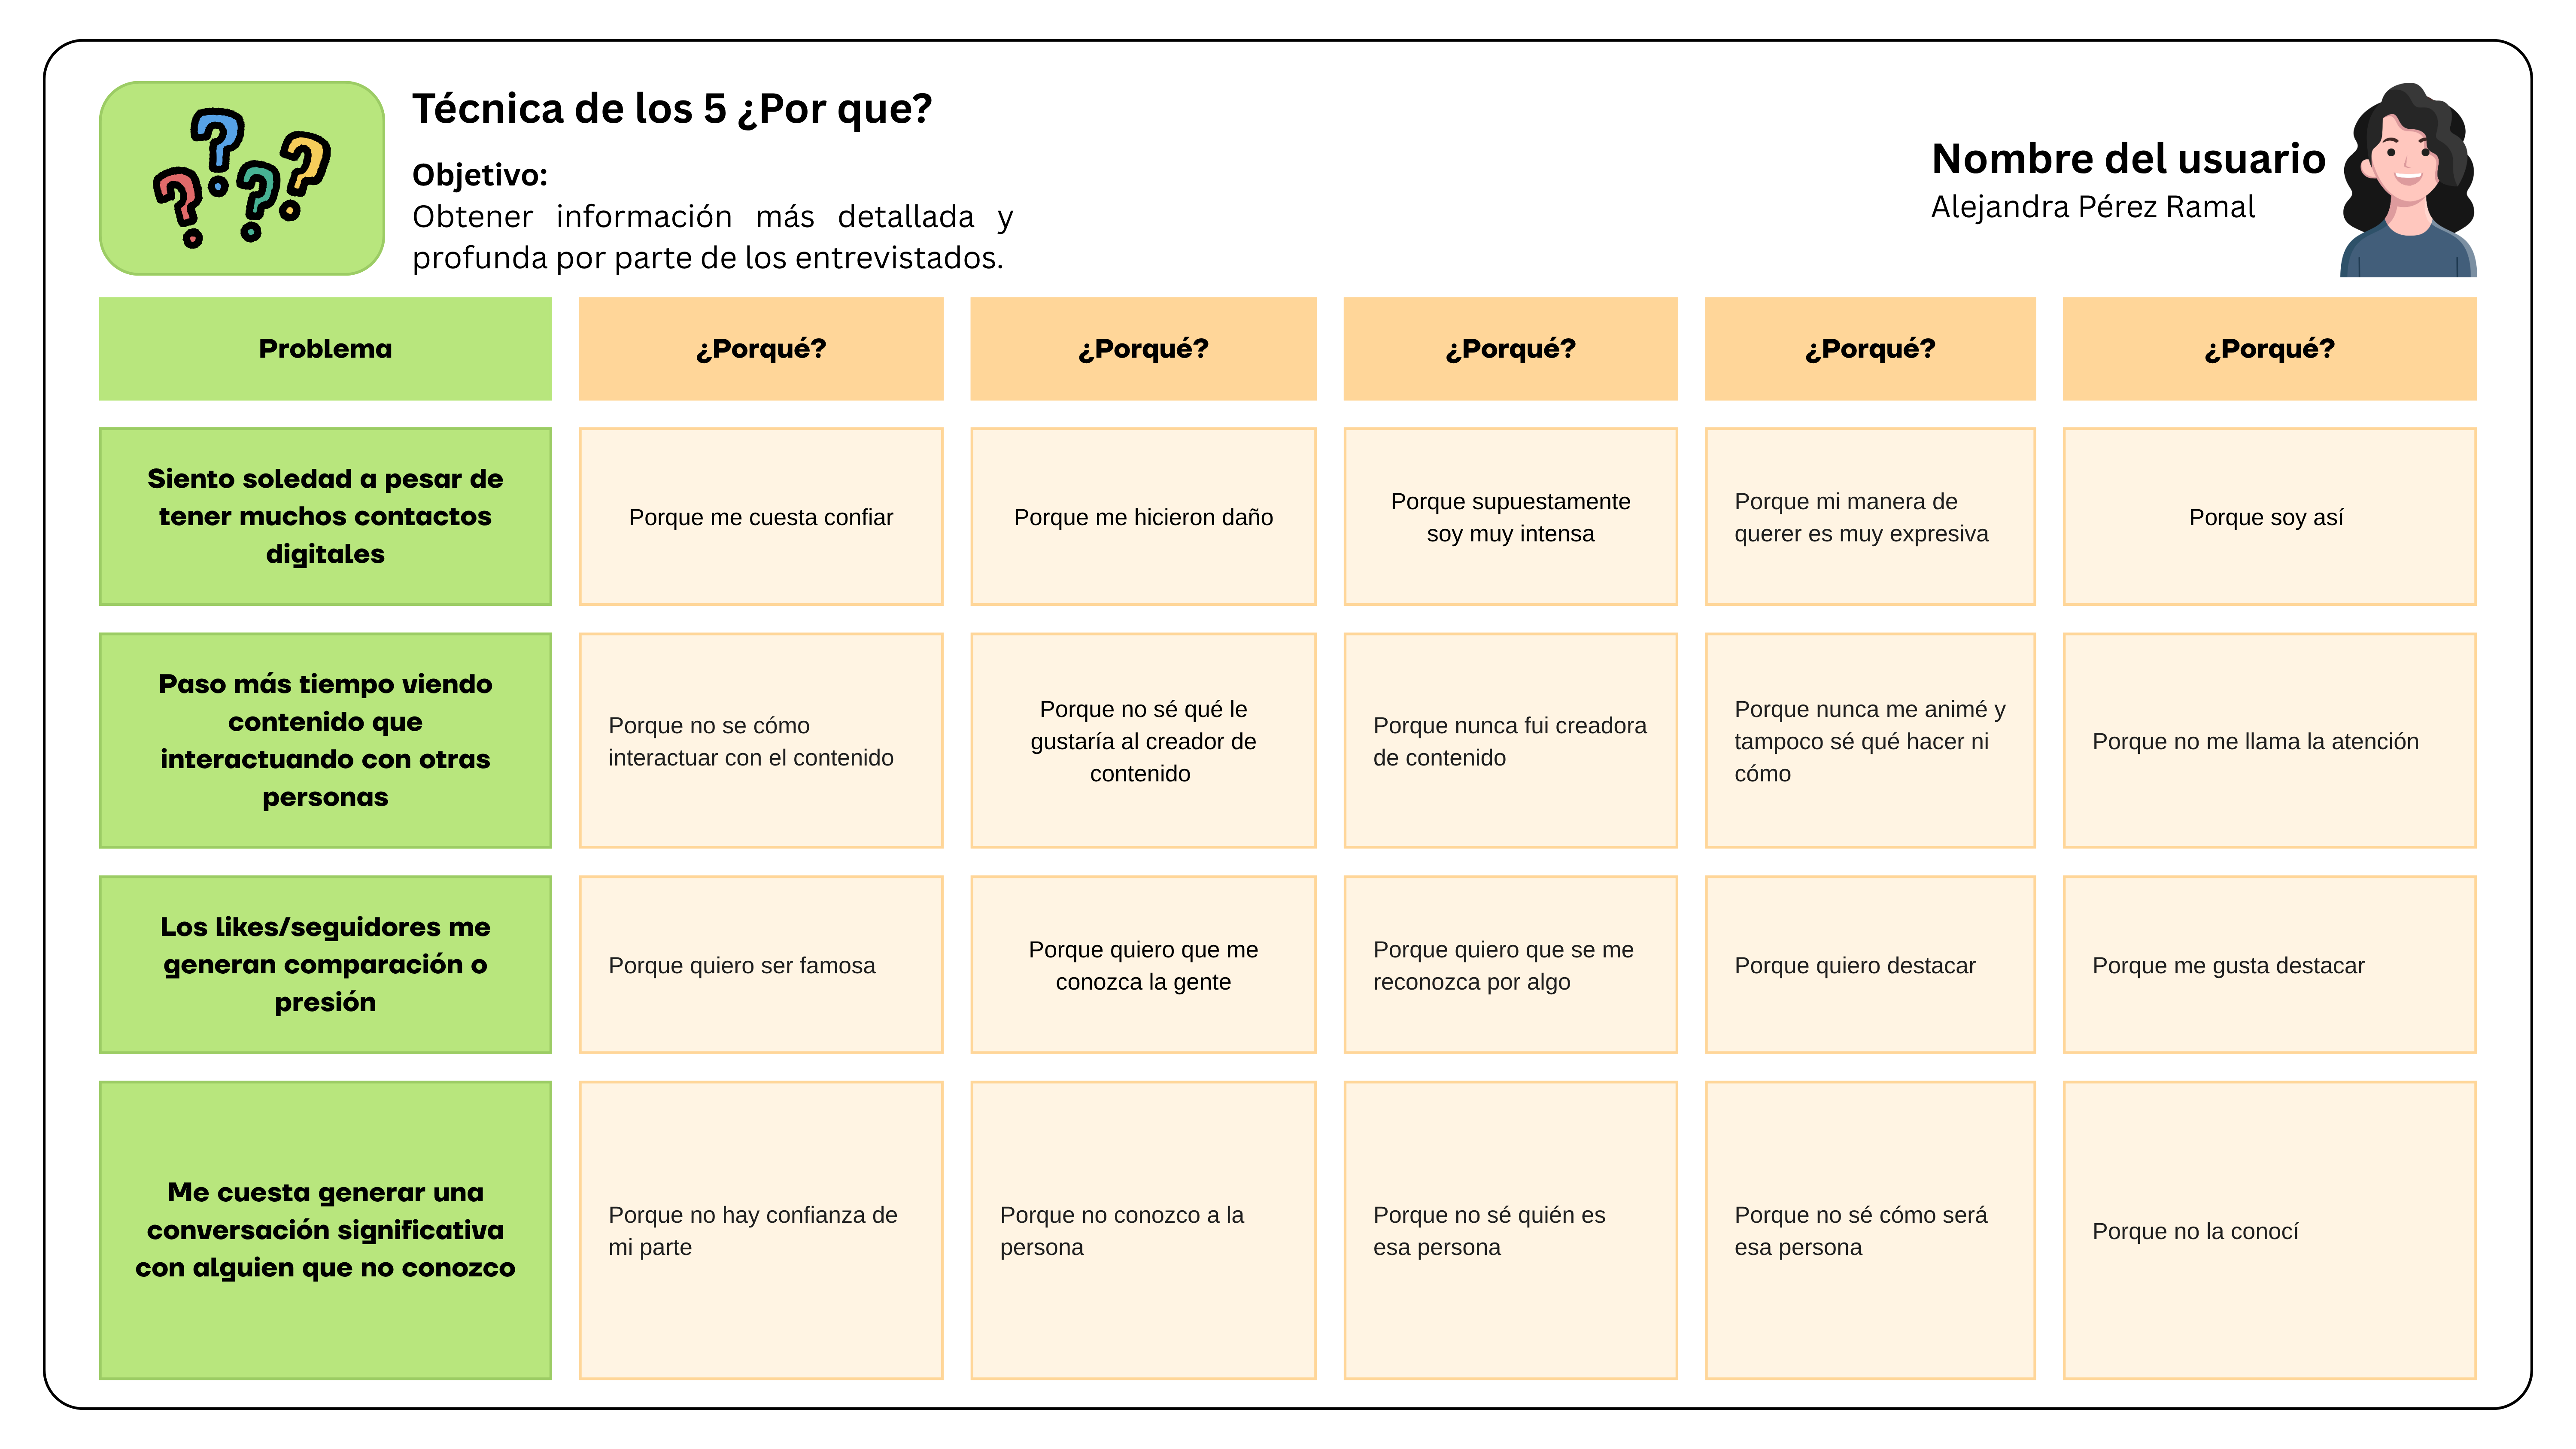
\includegraphics[width=0.9\textwidth]{Images/methodology/empathy/usuario5-5P.png}
  \vspace{4pt}
\end{figure}

En este caso, la causa raíz identificada se vincula a experiencias previas de conflicto derivadas de una forma intensa y expresiva de relacionarse, lo que ha generado cierta cautela al momento de establecer nuevos vínculos digitales. Este hallazgo resulta consistente con los procesos de regulación emocional descritos por Gross (1998), particularmente en lo referido a la modulación de la respuesta tras experiencias emocionalmente intensas.

\subsection{Usuarios 2, 3, 4 y 6}
El mismo análisis fue aplicado a los Usuarios 2 (Rubén Hernández Torrez), 3 (Fernando José Pérez Armando), 4 (Antonia Tapia) y 6 (Renata Martínez Mitte). En conjunto, las causas raíz identificadas a través de esta técnica coinciden en tres ejes: la falta de confianza inicial hacia desconocidos, la ausencia de un tema o interés en común que facilite el inicio de la conversación, y el temor a ser juzgado o rechazado al exponerse emocionalmente. Estos ejes son coherentes con la caracterización de la soledad como discrepancia entre las relaciones deseadas y las disponibles (Hawkley \& Cacioppo, 2010), y con la noción de "ilusión de amistad significativa en línea" documentada por Parry et al. (2026).

\section{SÍNTESIS DE LA FASE EMPATIZAR}
La aplicación de las técnicas descritas en el presente capítulo permitió confirmar, desde la evidencia primaria, los factores identificados previamente a partir de la literatura en el Capítulo 3. De manera consistente entre los seis participantes, se evidenció: (a) la existencia de vínculos digitales numerosos pero de bajo significado emocional, en línea con Smith et al. (2021) y Takano (2018); (b) una fuerte preferencia por el emparejamiento basado en intereses o gustos compartidos como facilitador de la conversación, consistente con Liu et al. (2026); (c) una valoración positiva del uso de avatares como medio de expresión frente a la exposición de la identidad real; y (d) una necesidad explícita de mecanismos que generen confianza y seguridad frente a la interacción con desconocidos. Estos hallazgos constituyen la base para la construcción del planteamiento del problema y la definición del punto de vista de diseño que se desarrolla en el Capítulo 5.